% begin module area-between-curves-def
\begin{frame}[t]
\begin{tabular}{|c|c|}
\hline
 \ \ \ \ \ The Area Under a Curve \ \ \ \ \ &
 \ \ \ \ The Area Between Two Curves \ \ \ \ \\
\ \only<1>{%
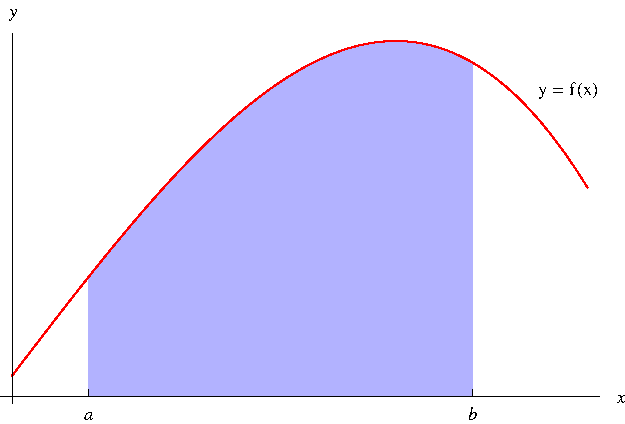
\includegraphics[height=3cm]{area-between-curves/pictures/06-01-singleint.pdf}%
}%
\only<handout:0| 2->{%
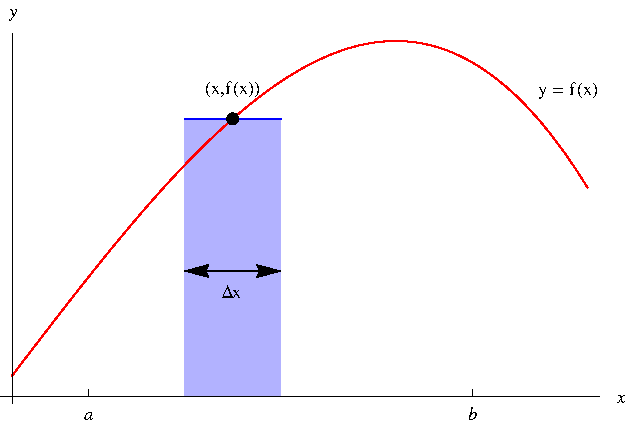
\includegraphics[height=3cm]{area-between-curves/pictures/06-01-1rectangle.pdf}%
}&%
\ \only<-12>{%
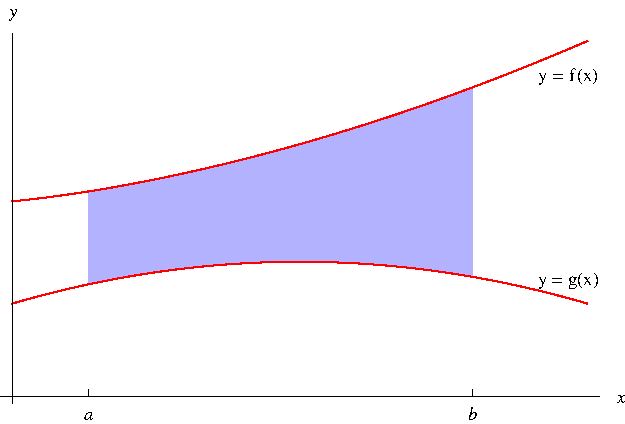
\includegraphics[height=3cm]{area-between-curves/pictures/06-01-doubleint.pdf}%
}%
\only<handout:0| 13->{%
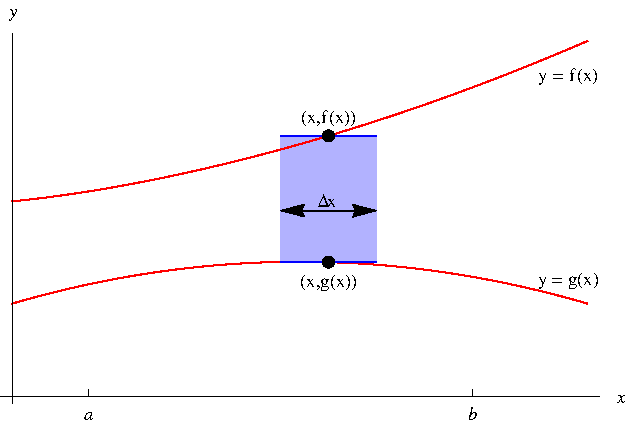
\includegraphics[height=3cm]{area-between-curves/pictures/06-01-1rectanglediff.pdf}%
}\\%
\uncover<2->{
rectangle area $ = $ \only<handout:0| -5>{\alert<handout:0| 5>{height}}\only<6->{\alert<handout:0| 6>{$f(x)$}}$\cdot$\only<handout:0| -3>{\alert<handout:0| 3>{width}}\only<4->{\alert<handout:0| 4>{$\Delta x$}}
} &
\uncover<13->{
rectangle area $ = $ \only<handout:0| -16>{\alert<handout:0| 16>{height}}\only<17->{\alert<handout:0| 17>{$(f(x)-g(x))$}}$\cdot$\only<handout:0| -14>{\alert<handout:0| 14>{width}}\only<15->{\alert<handout:0| 15>{$\Delta x$}}
} \\
\ \only<-7>{%
\uncover<7>{%
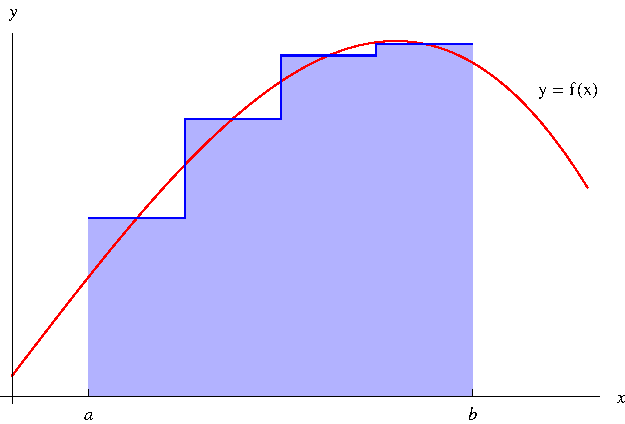
\includegraphics[height=3cm]{area-between-curves/pictures/06-01-4rectangle.pdf}%
}%
}%
\only<handout:0| 8>{%
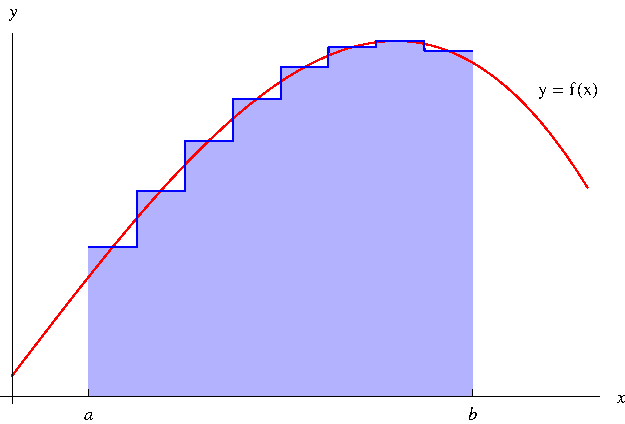
\includegraphics[height=3cm]{area-between-curves/pictures/06-01-8rectangle.pdf}%
}% 
\only<handout:0| 9>{%
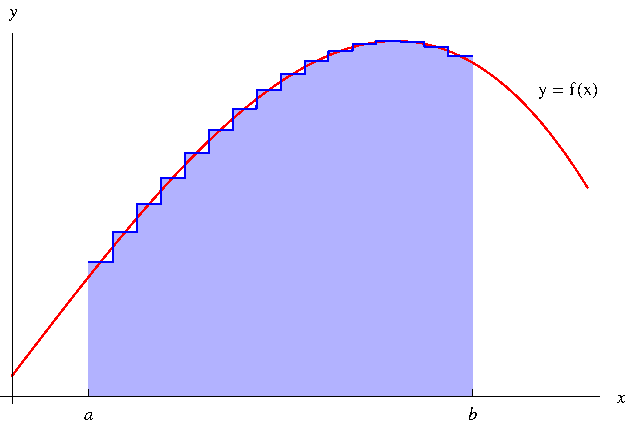
\includegraphics[height=3cm]{area-between-curves/pictures/06-01-16rectangle.pdf}%
}% 
\only<handout:0| 10->{%
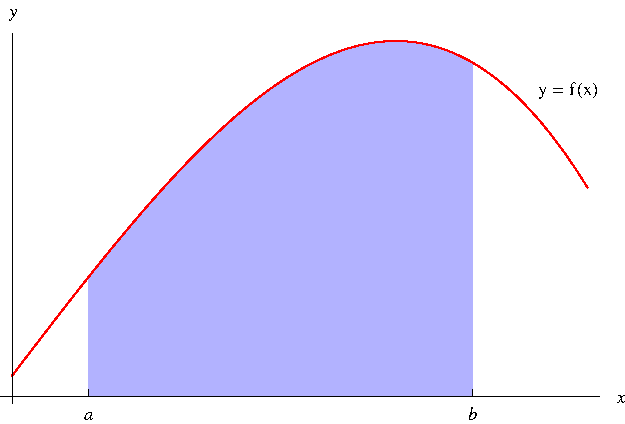
\includegraphics[height=3cm]{area-between-curves/pictures/06-01-singleint.pdf}%
}&%
\ \only<-18>{%
\uncover<18->{%
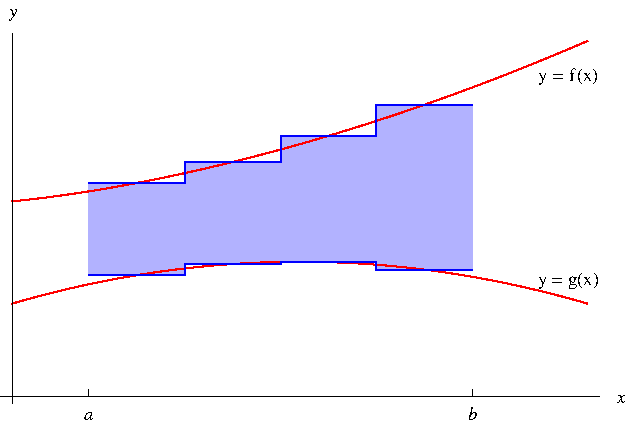
\includegraphics[height=3cm]{area-between-curves/pictures/06-01-4rectanglediff.pdf}%
}%
}%
\only<handout:0| 19>{%
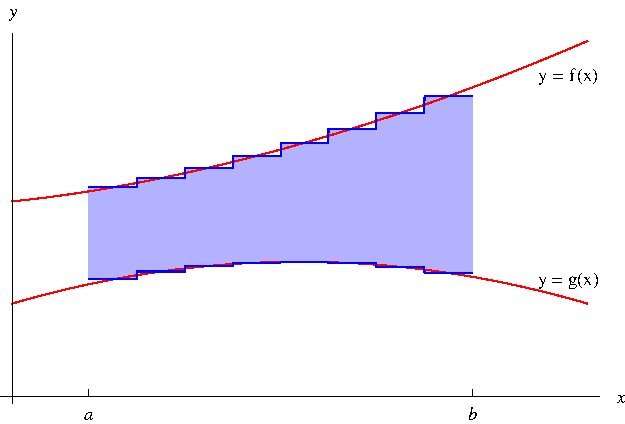
\includegraphics[height=3cm]{area-between-curves/pictures/06-01-8rectanglediff.pdf}%
}%  
\only<handout:0| 20>{%
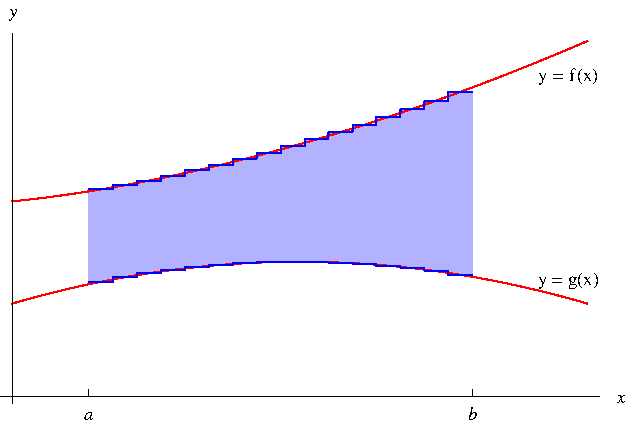
\includegraphics[height=3cm]{area-between-curves/pictures/06-01-16rectanglediff.pdf}%
}%  
\only<handout:0| 21>{%
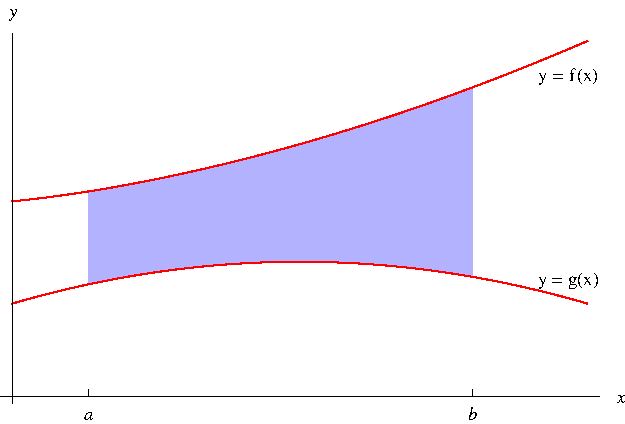
\includegraphics[height=3cm]{area-between-curves/pictures/06-01-doubleint.pdf}%
}\\
\uncover<7->{
\# rectangles $ = \alert<handout:0| 10>{n} \only<handout:0| -9>{=}\only<10->{\alert<handout:0| 10>{\rightarrow}} $ \only<handout:0| -7>{4}\only<handout:0| 8>{\alert<handout:0| 8>{8}}\only<handout:0| 9>{\alert<handout:0| 9>{16}}\only<10->{\alert<handout:0| 10>{$\infty$}}
} & 
\uncover<18->{
\# rectangles $ = n \only<handout:0| -20>{=}\only<21->{\rightarrow} $ \only<handout:0| -18>{4}\only<handout:0| 19>{8}\only<handout:0| 20>{16}\only<21->{$\infty$}
} \\
\only<handout:0| -9,12->{\invisible<1->{$\underset{n\rightarrow \infty}{\lim}$}}%
\uncover<7->{
A  =  \only<handout:0| 10-11>{\alert<handout:0| 10-11>{$\underset{n\rightarrow \infty}{\lim}$}}\only<handout:0| -11>{\alert<handout:0| 11>{$ \sum_{i = 1}^{\only<handout:0| -7>{4}\only<handout:0| 8>{\alert<handout:0| 8>{8}}\only<handout:0| 9>{\alert<handout:0| 9>{16}}\only<handout:0| 10->{\alert<handout:0| 10>{n}}} f(x_i)\Delta x$}}
\only<12->{\alert<handout:0| 12>{$ \int_a^b f(x)\diff x$}}
}% 
\only<-11>{\invisible<1->{$\int_a^b$}}%
& 
\uncover<18->{
A  =  \only<handout:0| -20>{$ \sum_{i = 1}^{\only<handout:0| -18>{4}\only<handout:0| 19>{8}\only<handout:0| 20>{16}} (f(x_i)- g(x_i))\Delta x$}
\only<21->{$ \int_a^b [f(x) - g(x)]\diff x$}
} \\ 
\hline
\end{tabular}
\end{frame}


\begin{frame}
\begin{definition}[The Area Between Two Curves]
The area between two curves $y = f(x)$ and $y = g(x)$ bounded by the endpoints $x = a$ and $x = b$ is
\[ \int_a^b |f(x) - g(x)|\diff x . \]

Note that we use the absolute value, because in general we don't know which curve is above the other.
\end{definition}
\end{frame}
% end module area-between-curves-def
